\documentclass{article}

% Language setting
% Replace `english' with e.g. `spanish' to change the document language
\usepackage[portuguese]{babel}

% Set page size and margins
% Replace `letterpaper' with `a4paper' for UK/EU standard size
\usepackage[letterpaper,top=2cm,bottom=2cm,left=3cm,right=3cm,marginparwidth=1.75cm]{geometry}

% Useful packages
\usepackage{amsmath}
\usepackage{graphicx}
\usepackage[colorlinks=true, allcolors=blue]{hyperref}

\title{Relatório do EP 3 de MAC0209}
\author{Andre Luis Neves - 15493840 \\ Joao Victor Alonso de Mello - 10951790 \\ Luis Claudio Vergara 15472544}

\begin{document}
\maketitle


\begin{abstract}
  Nesse EP, medimos o RSSI do WiFi nos entornos do IME-USP. Usamos esses dados para analisar as sombras de sinal de WiFi do Eduroam presentes na região.
  
  O vídeo mostrando o experimento está disponível \href{https://youtube.com}{aqui}.

\end{abstract}

\newpage

\tableofcontents

\newpage

\section{Introdução}
O WiFi é uma ferramenta essencial nas universidades. Dessa forma, manter uma boa intensidade de sinal no campus é de bastante importante, tanto para os professores quanto para os alunos, auxiliando em aulas e pesquisas.

Em particular, o IME teve vários investimentos nessa área nos últimos anos. Para conseguir maximizar a eficiência desses gastos, são necessários estudos e coleta de dados.

Assim, esse experimento visa mostrar potenciais sombras de WiFi do Eduroam, o que ajuda a identificar os melhores pontos para se colocar repetidoras de sinal.

\section{Objetivos}
O objetivo principal desse projeto é coletar dados e processá-los para entender quais pontos em torno do IME o sinal de WiFi e aqueles pontos onde há problemas de conexão.

Assim, é dividido em duas etapas: coleta de dados do RSSI e do GPS, e análise dos dados por meio de \textit{heatmaps} e gráficos de RSSI ao longo do tempo.

\section{Cronograma}

Começamos o trabalho no dia da gravação inicial dos vídeos, dia 09/06. A partir disso, definimos o cronograma com os prazos da seguinte forma:

\begin{itemize}
    \item Código inicial para testar o plot dos mapas: 16/06
    \item Coleta oficial dos dados com o professor: 16/06
    \item Versão finalizada do código e do vídeo: 28/06
    \item Escrita do relatório: 02/07
\end{itemize}

\section{Dados e métodos}
A aquisição de dados foi feita por meio do aplicativo do projeto SideSeeing, usando um colete acoplado ao celular.

Caminhamos em conjunto com outras pessoas que também estavam coletando dados ao redor do IME em três rotas distintas, a saber: ao redor do quarteirão do IME, ao redor dos blocos A, B e C, e dentro desses blocos.

A análise de dados produz um heatmap, um gráfico do RSSI ao longo do tempo, um gráfico de média dinâmica do RSSI nas proximidades de cada lugar e retorna a média e desvio padrão da intensidade do sinal ao longo de cada rota. A implementação detalhada do código para análise de dados pode ser encontrada no Jupiter Notebook.

\section{Resultados experimentais}
Ver Figuras 1,2,3.  

\begin{figure}
  \begin{center}
    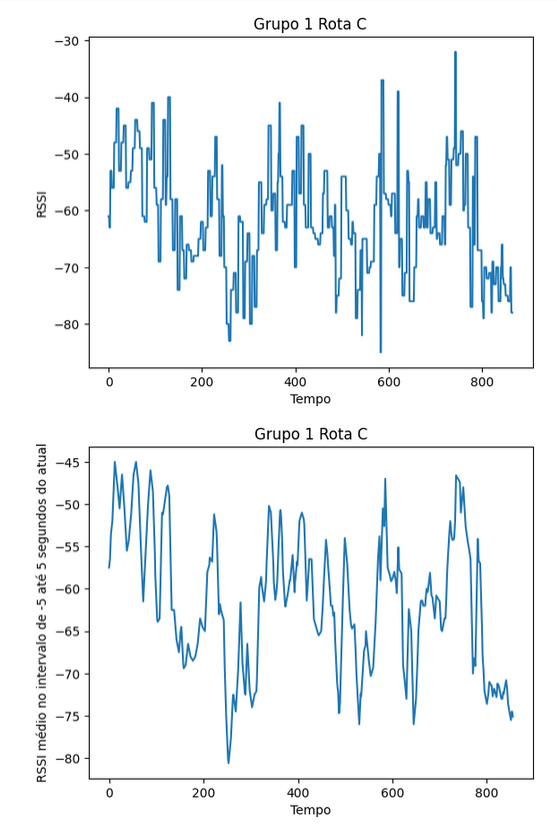
\includegraphics[width=0.95\textwidth]{figures/grupo_1-rota_c}
  \end{center}
  \caption{Grupo 1 Rota C}\label{fig:grupo_1-rota_c}
\end{figure}

\begin{figure}
  \begin{center}
    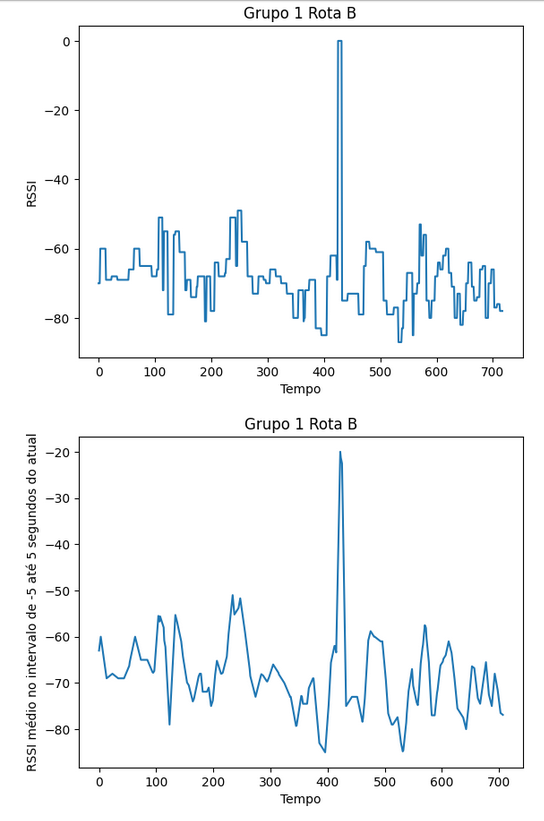
\includegraphics[width=0.95\textwidth]{figures/grupo_1-rota_b}
  \end{center}
  \caption{}\label{fig:}
\end{figure}

\begin{figure}
  \begin{center}
    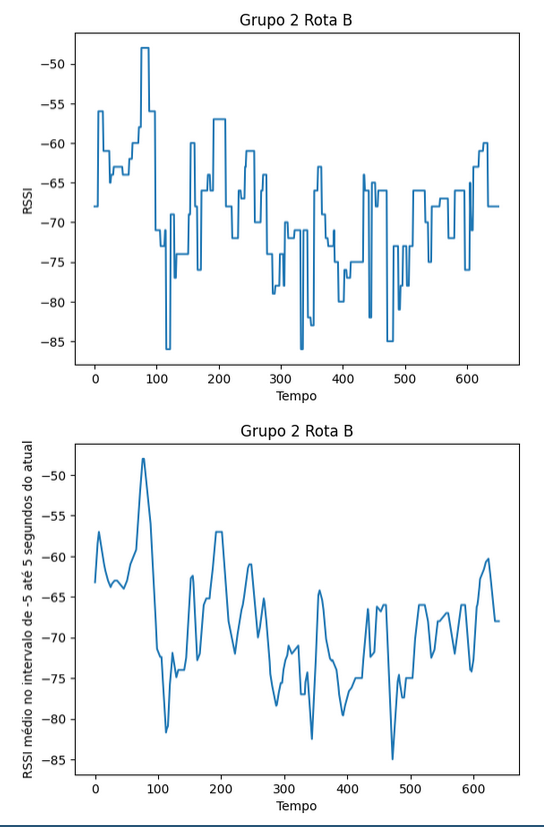
\includegraphics[width=0.95\textwidth]{figures/grupo_2-rota_b}
  \end{center}
  \caption{}\label{fig:}
\end{figure}

\section{Discussão e Conclusão}

A cobertura da rede Eduroam mostrou-se adequada dentro dos prédios do instituto e seguiu padrões esperados em seus arredores. A seção com menor intensidade de sinal foi a Travessa  V, enquanto que as áreas perto dos prédios principais (edifício Vila Nova Artigas, IME - bloco A e B, CCSL) possuíram a melhor cobertura de sinal. Porém, apesar do sinal ser forte dentro dos prédios, do lado de fora, mesmo logo ao lado deles, a intensidade cai drasticamente. Contudo, esse comportamento é esperado, considerando a grossura das paredes do instituto. Em conclusão, há uma boa cobertura WiFi nas áreas mais importantes do IME, mas tal cobertura não se estende para as áreas ao ar livre.

\end{document}
